\documentclass[10pt,sigconf,anonymous]{acmart}

\settopmatter{printacmref=false, printccs=false, printfolios=true}

\usepackage{booktabs} % For formal tables

\graphicspath{{figure/}{figures/}{Figure/}{Figures/}}

\usepackage{preamble}

% Copyright
\setcopyright{none}
%\setcopyright{acmcopyright}
%\setcopyright{acmlicensed}
% \setcopyright{rightsretained}
%\setcopyright{usgov}
%\setcopyright{usgovmixed}
%\setcopyright{cagov}
%\setcopyright{cagovmixed}


% DOI
\acmDOI{10.475/123_4}

% ISBN
\acmISBN{123-4567-24-567/08/06}

%Conference
\acmConference[SHORTNAME'23]{ACM Long Conference Name conference}{July 1997}{City, State, Country} 
\acmYear{2023}
\copyrightyear{2023}

\acmPrice{15.00}


\begin{document}
\title{SIG Proceedings Paper in LaTeX Format}
\titlenote{Produces the permission block, and copyright information}
% \subtitle{Paper \#, XXX pages}

\author{Firstname Lastname}
\authornote{Note}
\orcid{1234-5678-9012}
\affiliation{%
  \institution{Affiliation}
  \streetaddress{Address}
  \city{City}
  \state{State}
  \postcode{Zipcode}
}
\email{email@domain.com}

\author{Firstname Lastname}
\orcid{1234-5678-9012}
\affiliation{%
  \institution{Affiliation}
  \streetaddress{Address}
  \city{City}
  \state{State}
  \postcode{Zipcode}
}
\email{email@domain.com}

\author{Firstname Lastname}
\orcid{1234-5678-9012}
\affiliation{%
  \institution{Affiliation}
}
\email{email@domain.com}

\author{Firstname Lastname}
\orcid{1234-5678-9012}
\affiliation{%
  \institution{Affiliation}
}
\email{email@domain.com}

\author{Firstname Lastname}
\orcid{1234-5678-9012}
\affiliation{%
  \institution{Affiliation}
}
\email{email@domain.com}

% The default list of authors is too long for headers}
\renewcommand{\shortauthors}{F. Lastname et al.}

\begin{abstract}
  This paper provides a sample of a \LaTeX\ document which conforms,
  somewhat loosely, to the formatting guidelines for
  ACM SIG Proceedings.\footnote{This is an abstract footnote}
\end{abstract}

%
% The code below should be generated by the tool at
% http://dl.acm.org/ccs.cfm
% Please copy and paste the code instead of the example below. 
%
\begin{CCSXML}
  <ccs2012>
  <concept>
  <concept_id>10010520.10010553.10010562</concept_id>
  <concept_desc>Computer systems organization~Embedded systems</concept_desc>
  <concept_significance>500</concept_significance>
  </concept>
  <concept>
  <concept_id>10010520.10010575.10010755</concept_id>
  <concept_desc>Computer systems organization~Redundancy</concept_desc>
  <concept_significance>300</concept_significance>
  </concept>
  <concept>
  <concept_id>10010520.10010553.10010554</concept_id>
  <concept_desc>Computer systems organization~Robotics</concept_desc>
  <concept_significance>100</concept_significance>
  </concept>
  <concept>
  <concept_id>10003033.10003083.10003095</concept_id>
  <concept_desc>Networks~Network reliability</concept_desc>
  <concept_significance>100</concept_significance>
  </concept>
  </ccs2012>
\end{CCSXML}

\ccsdesc[500]{Computer systems organization~Embedded systems}
\ccsdesc[300]{Computer systems organization~Redundancy}
\ccsdesc{Computer systems organization~Robotics}
\ccsdesc[100]{Networks~Network reliability}

% We no longer use \terms command
%\terms{Theory}

\keywords{ACM proceedings}

\maketitle

\PageGlossariesfalse
% \include{TexFiles/Glossary}

\section{Introduction}

Refer to \verb|acmart.pdf| \cite{veytsmanlatex} (\url{https://www.ctan.org/pkg/acmart}, \url{http://www.acm.org/publications/proceedings-template}) for additional examples and instructions.

\subsection{Subsection}

Lorem ipsum dolor sit amet, consectetur \alltoall \allreduce adipiscing elit. 
Sed aliquam nisl turpis, sit amet mollis leo accumsan vel. \mpi
Donec semper turpis dui, a porttitor lorem tincidunt id.
Phasellus gravida, purus non faucibus euismod, lectus tortor maximus elit, vestibulum lobortis purus turpis non urna.
Fusce feugiat lectus ut massa molestie, non interdum augue porta.
Nunc dapibus odio nec neque cursus, ut lacinia velit rutrum.
Duis tempor nulla velit, sed pellentesque nunc imperdiet ut.
Phasellus eget hendrerit neque.
Suspendisse aliquet nulla id sem aliquam aliquam sed a orci.
Duis sem est, hendrerit nec porttitor sit amet, maximus sed nulla.
Suspendisse et dictum massa.
Morbi non diam nec orci sodales eleifend.
Etiam eget finibus purus, a malesuada ipsum.
Nullam ac nisi nec elit faucibus aliquet.
Nulla feugiat velit sed sodales eleifend.
Donec orci nulla, viverra et mi in, sagittis egestas urna.

\begin{figure}[htbp]
  \centering
  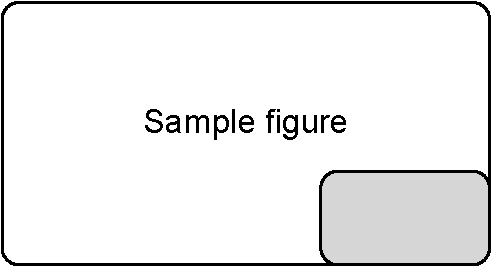
\includegraphics[scale=0.5]{sample-figure}
  \caption{Sample figure}
  \label{fig1:../Figures/sample}
\end{figure}

\subsubsection{Subsubsection}

Integer eleifend quam et odio iaculis, at elementum augue aliquam.
Ut eu nibh nec urna finibus semper fermentum id purus.
Aliquam eu sollicitudin libero.
Cras viverra elit congue erat pulvinar, vitae vehicula tortor interdum.
Aliquam commodo mi sapien, ullamcorper egestas velit tempor nec.
Quisque sapien velit, fringilla non vulputate nec, lacinia in dui.
Nam vestibulum volutpat ante, eu sodales enim tincidunt vel.
Ut mollis elit quis bibendum eleifend.
In laoreet tortor non odio ultrices mollis.
Curabitur volutpat et risus quis fermentum.
Morbi laoreet ligula eget orci consectetur, in dictum ipsum efficitur.
Mauris nec neque ultricies, efficitur elit id, hendrerit nibh.
Interdum et malesuada fames ac ante ipsum primis in faucibus.

\paragraph{Paragraph}

Nulla scelerisque id lectus a luctus.
Curabitur quis dolor maximus, maximus erat ut, placerat justo.
Donec auctor purus a lacus molestie maximus.
Etiam porta ligula a quam mollis efficitur.
Quisque vel sapien iaculis, pellentesque lorem nec, hendrerit lectus.
Vestibulum egestas congue euismod.
Praesent a tristique massa.
Aliquam eget ante elit.
Phasellus eget metus mi.
Fusce nec rutrum mi.
Pellentesque eu congue mi.
Fusce eu ullamcorper est.

\section{Background}

Refer to \verb|acmart.pdf| \cite{veytsmanlatex} (\url{https://www.ctan.org/pkg/acmart}, \url{http://www.acm.org/publications/proceedings-template}) for additional examples and instructions.

\subsection{Subsection}

Lorem ipsum dolor sit amet, consectetur adipiscing elit.
Sed aliquam nisl turpis, sit amet mollis leo accumsan vel.
Donec semper turpis dui, a porttitor lorem tincidunt id.
Phasellus gravida, purus non faucibus euismod, lectus tortor maximus elit, vestibulum lobortis purus turpis non urna.
Fusce feugiat lectus ut massa molestie, non interdum augue porta.
Nunc dapibus odio nec neque cursus, ut lacinia velit rutrum.
Duis tempor nulla velit, sed pellentesque nunc imperdiet ut.
Phasellus eget hendrerit neque.
Suspendisse aliquet nulla id sem aliquam aliquam sed a orci.
Duis sem est, hendrerit nec porttitor sit amet, maximus sed nulla.
Suspendisse et dictum massa.
Morbi non diam nec orci sodales eleifend.
Etiam eget finibus purus, a malesuada ipsum.
Nullam ac nisi nec elit faucibus aliquet.
Nulla feugiat velit sed sodales eleifend.
Donec orci nulla, viverra et mi in, sagittis egestas urna.

\begin{figure}[htbp]
  \centering
  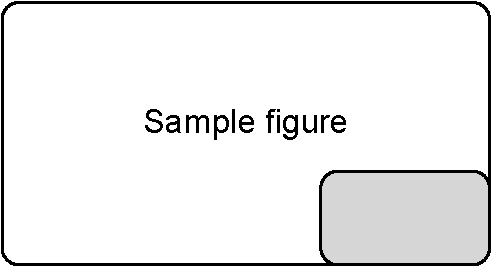
\includegraphics[scale=0.5]{sample-figure}
  \caption{Sample figure}
  \Description{Sample figure description.}
  \label{fig2:../Figures/sample}
\end{figure}

\subsubsection{Subsubsection}

Integer eleifend quam et odio iaculis, at elementum augue aliquam.
Ut eu nibh nec urna finibus semper fermentum id purus.
Aliquam eu sollicitudin libero.
Cras viverra elit congue erat pulvinar, vitae vehicula tortor interdum.
Aliquam commodo mi sapien, ullamcorper egestas velit tempor nec.
Quisque sapien velit, fringilla non vulputate nec, lacinia in dui.
Nam vestibulum volutpat ante, eu sodales enim tincidunt vel.
Ut mollis elit quis bibendum eleifend.
In laoreet tortor non odio ultrices mollis.
Curabitur volutpat et risus quis fermentum.
Morbi laoreet ligula eget orci consectetur, in dictum ipsum efficitur.
Mauris nec neque ultricies, efficitur elit id, hendrerit nibh.
Interdum et malesuada fames ac ante ipsum primis in faucibus.

\paragraph{Paragraph}

Nulla scelerisque id lectus a luctus.
Curabitur quis dolor maximus, maximus erat ut, placerat justo.
Donec auctor purus a lacus molestie maximus.
Etiam porta ligula a quam mollis efficitur.
Quisque vel sapien iaculis, pellentesque lorem nec, hendrerit lectus.
Vestibulum egestas congue euismod.
Praesent a tristique massa.
Aliquam eget ante elit.
Phasellus eget metus mi.
Fusce nec rutrum mi.
Pellentesque eu congue mi.
Fusce eu ullamcorper est.

\section{Proposal}

Refer to \verb|acmart.pdf| \cite{veytsmanlatex} (\url{https://www.ctan.org/pkg/acmart}, \url{http://www.acm.org/publications/proceedings-template}) for additional examples and instructions.

\subsection{Subsection}

Lorem ipsum dolor sit amet, consectetur adipiscing elit.
Sed aliquam nisl turpis, sit amet mollis leo accumsan vel.
Donec semper turpis dui, a porttitor lorem tincidunt id.
Phasellus gravida, purus non faucibus euismod, lectus tortor maximus elit, vestibulum lobortis purus turpis non urna.
Fusce feugiat lectus ut massa molestie, non interdum augue porta.
Nunc dapibus odio nec neque cursus, ut lacinia velit rutrum.
Duis tempor nulla velit, sed pellentesque nunc imperdiet ut.
Phasellus eget hendrerit neque.
Suspendisse aliquet nulla id sem aliquam aliquam sed a orci.
Duis sem est, hendrerit nec porttitor sit amet, maximus sed nulla.
Suspendisse et dictum massa.
Morbi non diam nec orci sodales eleifend.
Etiam eget finibus purus, a malesuada ipsum.
Nullam ac nisi nec elit faucibus aliquet.
Nulla feugiat velit sed sodales eleifend.
Donec orci nulla, viverra et mi in, sagittis egestas urna.

\begin{figure}[htbp]
  \centering
  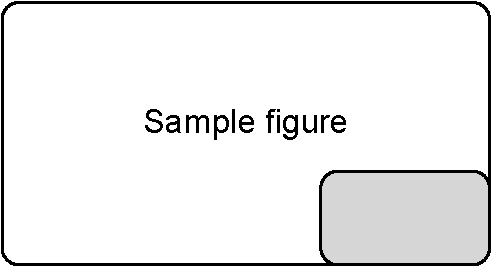
\includegraphics[scale=0.5]{sample-figure}
  \caption{Sample figure}
  \Description{Sample figure description.}
  \label{fig3:../Figures/sample}
\end{figure}

\subsubsection{Subsubsection}

Integer eleifend quam et odio iaculis, at elementum augue aliquam.
Ut eu nibh nec urna finibus semper fermentum id purus.
Aliquam eu sollicitudin libero.
Cras viverra elit congue erat pulvinar, vitae vehicula tortor interdum.
Aliquam commodo mi sapien, ullamcorper egestas velit tempor nec.
Quisque sapien velit, fringilla non vulputate nec, lacinia in dui.
Nam vestibulum volutpat ante, eu sodales enim tincidunt vel.
Ut mollis elit quis bibendum eleifend.
In laoreet tortor non odio ultrices mollis.
Curabitur volutpat et risus quis fermentum.
Morbi laoreet ligula eget orci consectetur, in dictum ipsum efficitur.
Mauris nec neque ultricies, efficitur elit id, hendrerit nibh.
Interdum et malesuada fames ac ante ipsum primis in faucibus.

\paragraph{Paragraph}

Nulla scelerisque id lectus a luctus.
Curabitur quis dolor maximus, maximus erat ut, placerat justo.
Donec auctor purus a lacus molestie maximus.
Etiam porta ligula a quam mollis efficitur.
Quisque vel sapien iaculis, pellentesque lorem nec, hendrerit lectus.
Vestibulum egestas congue euismod.
Praesent a tristique massa.
Aliquam eget ante elit.
Phasellus eget metus mi.
Fusce nec rutrum mi.
Pellentesque eu congue mi.
Fusce eu ullamcorper est.

\section{Results}

Refer to \verb|acmart.pdf| \cite{veytsmanlatex} (\url{https://www.ctan.org/pkg/acmart}, \url{http://www.acm.org/publications/proceedings-template}) for additional examples and instructions.

\subsection{Subsection}

Lorem ipsum dolor sit amet, consectetur adipiscing elit.
Sed aliquam nisl turpis, sit amet mollis leo accumsan vel.
Donec semper turpis dui, a porttitor lorem tincidunt id.
Phasellus gravida, purus non faucibus euismod, lectus tortor maximus elit, vestibulum lobortis purus turpis non urna.
Fusce feugiat lectus ut massa molestie, non interdum augue porta.
Nunc dapibus odio nec neque cursus, ut lacinia velit rutrum.
Duis tempor nulla velit, sed pellentesque nunc imperdiet ut.
Phasellus eget hendrerit neque.
Suspendisse aliquet nulla id sem aliquam aliquam sed a orci.
Duis sem est, hendrerit nec porttitor sit amet, maximus sed nulla.
Suspendisse et dictum massa.
Morbi non diam nec orci sodales eleifend.
Etiam eget finibus purus, a malesuada ipsum.
Nullam ac nisi nec elit faucibus aliquet.
Nulla feugiat velit sed sodales eleifend.
Donec orci nulla, viverra et mi in, sagittis egestas urna.

\begin{figure}[htbp]
  \centering
  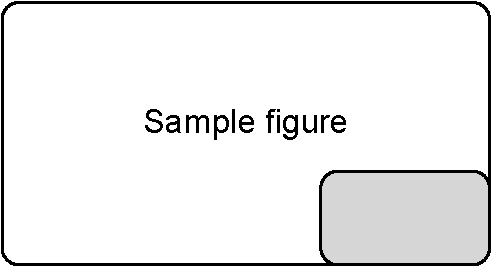
\includegraphics[scale=0.5]{sample-figure}
  \caption{Sample figure}
  \label{fig4:../Figures/sample}
\end{figure}

\subsubsection{Subsubsection}

Integer eleifend quam et odio iaculis, at elementum augue aliquam.
Ut eu nibh nec urna finibus semper fermentum id purus.
Aliquam eu sollicitudin libero.
Cras viverra elit congue erat pulvinar, vitae vehicula tortor interdum.
Aliquam commodo mi sapien, ullamcorper egestas velit tempor nec.
Quisque sapien velit, fringilla non vulputate nec, lacinia in dui.
Nam vestibulum volutpat ante, eu sodales enim tincidunt vel.
Ut mollis elit quis bibendum eleifend.
In laoreet tortor non odio ultrices mollis.
Curabitur volutpat et risus quis fermentum.
Morbi laoreet ligula eget orci consectetur, in dictum ipsum efficitur.
Mauris nec neque ultricies, efficitur elit id, hendrerit nibh.
Interdum et malesuada fames ac ante ipsum primis in faucibus.

\paragraph{Paragraph}

Nulla scelerisque id lectus a luctus.
Curabitur quis dolor maximus, maximus erat ut, placerat justo.
Donec auctor purus a lacus molestie maximus.
Etiam porta ligula a quam mollis efficitur.
Quisque vel sapien iaculis, pellentesque lorem nec, hendrerit lectus.
Vestibulum egestas congue euismod.
Praesent a tristique massa.
Aliquam eget ante elit.
Phasellus eget metus mi.
Fusce nec rutrum mi.
Pellentesque eu congue mi.
Fusce eu ullamcorper est.

\section{Conclusions}

Refer to \verb|acmart.pdf| \cite{veytsmanlatex} (\url{https://www.ctan.org/pkg/acmart}, \url{http://www.acm.org/publications/proceedings-template}) for additional examples and instructions.

\subsection{Subsection}

Lorem ipsum dolor sit amet, consectetur adipiscing elit.
Sed aliquam nisl turpis, sit amet mollis leo accumsan vel.
Donec semper turpis dui, a porttitor lorem tincidunt id.
Phasellus gravida, purus non faucibus euismod, lectus tortor maximus elit, vestibulum lobortis purus turpis non urna.
Fusce feugiat lectus ut massa molestie, non interdum augue porta.
Nunc dapibus odio nec neque cursus, ut lacinia velit rutrum.
Duis tempor nulla velit, sed pellentesque nunc imperdiet ut.
Phasellus eget hendrerit neque.
Suspendisse aliquet nulla id sem aliquam aliquam sed a orci.
Duis sem est, hendrerit nec porttitor sit amet, maximus sed nulla.
Suspendisse et dictum massa.
Morbi non diam nec orci sodales eleifend.
Etiam eget finibus purus, a malesuada ipsum.
Nullam ac nisi nec elit faucibus aliquet.
Nulla feugiat velit sed sodales eleifend.
Donec orci nulla, viverra et mi in, sagittis egestas urna.

\begin{figure}[htbp]
  \centering
  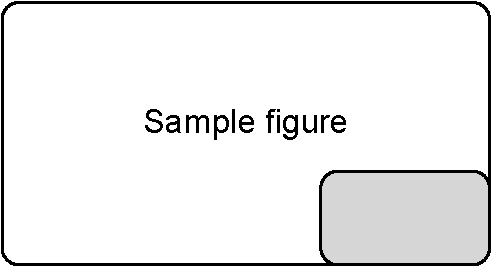
\includegraphics[scale=0.5]{sample-figure}
  \caption{Sample figure}
  \Description{Sample figure description.}
  \label{fig5:../Figures/sample}
\end{figure}

\subsubsection{Subsubsection}

Integer eleifend quam et odio iaculis, at elementum augue aliquam.
Ut eu nibh nec urna finibus semper fermentum id purus.
Aliquam eu sollicitudin libero.
Cras viverra elit congue erat pulvinar, vitae vehicula tortor interdum.
Aliquam commodo mi sapien, ullamcorper egestas velit tempor nec.
Quisque sapien velit, fringilla non vulputate nec, lacinia in dui.
Nam vestibulum volutpat ante, eu sodales enim tincidunt vel.
Ut mollis elit quis bibendum eleifend.
In laoreet tortor non odio ultrices mollis.
Curabitur volutpat et risus quis fermentum.
Morbi laoreet ligula eget orci consectetur, in dictum ipsum efficitur.
Mauris nec neque ultricies, efficitur elit id, hendrerit nibh.
Interdum et malesuada fames ac ante ipsum primis in faucibus.

\paragraph{Paragraph}

Nulla scelerisque id lectus a luctus.
Curabitur quis dolor maximus, maximus erat ut, placerat justo.
Donec auctor purus a lacus molestie maximus.
Etiam porta ligula a quam mollis efficitur.
Quisque vel sapien iaculis, pellentesque lorem nec, hendrerit lectus.
Vestibulum egestas congue euismod.
Praesent a tristique massa.
Aliquam eget ante elit.
Phasellus eget metus mi.
Fusce nec rutrum mi.
Pellentesque eu congue mi.
Fusce eu ullamcorper est.


\bibliographystyle{acm}
\bibliography{sigproc}

\end{document}
